\documentclass[11pt]{article}

\usepackage{latexsym}
\usepackage{amssymb}
\usepackage{amsthm}
\usepackage{graphicx}
\usepackage{enumerate}
\usepackage{amsmath}
\usepackage{cancel}
\numberwithin{equation}{section}

\setlength{\evensidemargin}{.25in}
\setlength{\oddsidemargin}{-.25in}
\setlength{\topmargin}{-.75in}
\setlength{\textwidth}{6.5in}
\setlength{\textheight}{9.5in}
\newcommand{\due}{September 30th, 2015}
\newcommand{\HWnum}{4}
\newcommand{\grad}{\bold\nabla}
\newcommand{\vecE}{\vec{E}}
\newcommand{\scrptR}{\vec{\mathfrak{R}}}
\newcommand{\kapa}{\frac{1}{4\pi\epsilon_0}}
\newcommand{\emf}{\mathcal{E}}
\newcommand{\unit}[1]{\ensuremath{\, \mathrm{#1}}}
\newcommand{\real}{\textnormal{Re}}
\newcommand{\Erf}{\textnormal{Erf}}
\newcommand{\sech}{\textnormal{sech}}
\newcommand{\scrO}{\mathcal{O}}
\newcommand{\levi}{\widetilde{\epsilon}}
\newcommand{\partiald}[2]{\ensuremath{\frac{\partial{#1}}{\partial{#2}}}}
\newcommand{\norm}[2]{\langle{#1}|{#2}\rangle}
\newcommand{\inprod}[2]{\langle{#1}|{#2}\rangle}
\newcommand{\ket}[1]{|{#1}\rangle}
\newcommand{\bra}[1]{\langle{#1}|}





\begin{document}
\begin{titlepage}
\setlength{\topmargin}{1.5in}
\begin{center}
\Huge{Physics 3320} \\
\LARGE{Principles of Electricity and Magnetism II} \\
\Large{Professor Ana Maria Rey} \\[1cm]

\huge{Homework \#\HWnum}\\[0.5cm]

\large{Joe Becker} \\
\large{SID: 810-07-1484} \\
\large{\due} 

\end{center}

\end{titlepage}



\section{Problem \#1}
For the integral 
$$\int_{0}^{(1+i)}\bar{z}dz$$
for $z\in\mathbb{C}$ we can test if the solution to this integral is path dependent by 
integrating over two different paths. For the first path we integrate over $C_1$ and $C_2$
where $C_1$ is along the real axes for $y=0, x$ and $C_2$ is along the line where $y,x=1$.
So,
\begin{align*}
\int_{0}^{(1+i)}\bar{z}dz &= \int_{C_1}\bar{z}dz + \int_{C_2}\bar{z}dz\\
&= \int_{0}^{1}dx(x-i0) + \int_{0}^{1}idy(1-iy)\\
&= \left.\frac{x^2}{2}\right|_0^1 + \int_{0}^{1}dy(i+y)\\
&= \frac{1}{2}-0 + \left.iy+\frac{y^2}{2}\right|_0^1\\
&= \frac{1}{2}-0 + (i+\frac{1}{2}-0)\\
&= 1+i
\end{align*}
Now we integrate over $C_3$ and $C_4$ where $C_3$ is the path along the imaginary axes for
$y,x=0$ and $C_4$ is the path where $y=1,x$. So we calculate
\begin{align*}
\int_{0}^{(1+i)}\bar{z}dz &= \int_{C_3}\bar{z}dz + \int_{C_4}\bar{z}dz\\
&= \int_0^1idy(0-iy) + \int_{0}^{1}dx(x-i)\\
&= \int_0^1ydy + \int_{0}^{1}(x-i)dx\\
&= \left.\frac{y^2}{2}\right|_0^1 + \left.\frac{x^2}{2}-ix\right|_{0}^{1}\\
&= \frac{1}{2}-0 + \frac{1^2}{2}-i-0\\
&= 1-i
\end{align*}
We see that the integral of $\bar{z}$ is path dependent.

\pagebreak

\section{Problem \#2}
For $u(x,y)=xy$ we can test if it is a harmonic function by calculating
$$\frac{\partial^2u}{\partial x^2} + \frac{\partial^2u}{\partial y^2} = y\frac{\partial^2}{\partial x^2}x + x\frac{\partial^2}{\partial y^2}y = 0$$ 
So we confirm that $u(x,y)$ is a harmonic function. To find the harmonic conjugate we 
construct a complex function $f=u+iv$ where $v(x,y)$ is a harmonic function that makes $f$
analytic. We can find $v$ by the \emph{Cauchy-Riemann} equations
\begin{align}
\partiald{}{x}u &= \partiald{}{y}v\\
\partiald{}{x}v &= -\partiald{}{y}u
\end{align}
Which yields
\begin{align*}
\partiald{}{y}v &= \partiald{}{x}(xy)\\
\partiald{}{y}v &= y\\
&\Downarrow\\
v(x,y) &= \frac{y^2}{2} + C(x)
\end{align*}
We find $C(x)$ by the other equation
\begin{align*}
\partiald{}{x}\left(\frac{y^2}{2}+C(x)\right) &= -\partiald{}{y}(xy)\\
C'(x) &= -x\\
&\Downarrow\\
C(x) &= -\frac{x^2}{2}
\end{align*}
So the harmonic conjugate of $u(x,y)$ is 
$$v(x,y) = \frac{y^2}{2} - \frac{x^2}{2}$$
Note that we test
$$\frac{\partial^2v}{\partial x^2} + \frac{\partial^2v}{\partial y^2} = \frac{\partial^2}{\partial x^2}\frac{-x^2}{2} + \frac{\partial^2}{\partial y^2}\frac{y^2}{2} =-1+1 =  0$$ 
so we confirm that $v(x,y)$ is harmonic. We can repeat this process for $u(x,y) = \cosh{x}\sin{y}$.
So we apply equations $2.1$ and $2.2$ to find $v(x,y)$
\begin{align*}
\partiald{v}{y} &= \sin{y}\partiald{}{x}\cosh{x}\\
\partiald{v}{y} &= \sin{y}\sinh{x}\\
&\Downarrow\\
v(x,y) &= -\cos{y}\sinh{x} + C(x)
\end{align*}
and
\begin{align*}
\partiald{v}{x} &= -\cosh{x}\partiald{}{y}\sin{y}\\
\partiald{v}{x} &= -\cosh{x}\cos{y}\\
-\cos{y}\cosh{x}+C'(x) &= -\cosh{x}\cos{y}\\
\end{align*}
So $C'(x)=0$ which implies that $C(x)$ is a constant. So we can write
$$v(x,y) = -\cos{y}\sinh{x}$$ 

\pagebreak

\section{Problem \#3}
\begin{enumerate}[(a)]
\item For the function $f=1/z$ where $z\in\mathbb{C}$. We want $f$ to be in the form of 
$f = u+iv$. We rationalize the denominator to do this
$$f= \frac{1}{z} = \frac{1}{x+iy}\frac{x-iy}{x-iy} = \frac{x-iy}{x^2+y^2} = \frac{x}{x^2+y^2} + i\frac{-y}{x^2+y^2}$$
So we can see that 
\begin{align*}
u(x,y) &= \frac{x}{x^2+y^2}\\
v(x,y) &= \frac{-y}{x^2+y^2}
\end{align*}
We can plot the level curves given by these functions. The result is shown in Figure 
\ref{Fig1}. Note that the curves of $u(x,y)$ are orthogonal to the curves of $v(x,y)$ which
implies that $f$ is analytic.
\begin{figure}
\centering
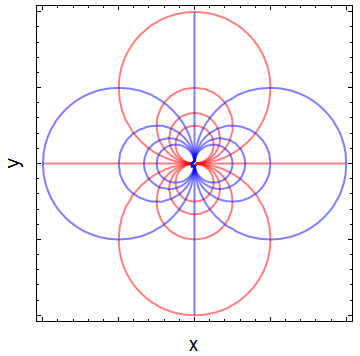
\includegraphics[width=0.75\textwidth]{Figure1.png}
\caption{Plot of level curves of $u(x,y)$ (in blue) and $v(x,y)$ (in red) for $f=1/z$.}
\label{Fig1}
\end{figure}

\item For $f=1/z^2$ where $z\in\mathbb{C}$ we want to rearrange into the form $f=u+iv$ by
\begin{align*}
\frac{1}{z^2} &= \frac{1}{(x+iy)^2}\\
&= \frac{1}{x^2-y^2+2ixy}\frac{x^2-y^2-2ixy}{x^2-y^2-2ixy}\\
&= \frac{x^2-y^2-2ixy}{x^4-x^2y^2+2ix^3y - x^2y^2+y^4-2ixy^3 - 2ix^3y+2ixy^3+4x^2y^2}\\
&= \frac{x^2-y^2-2ixy}{x^4-y^4+2x^2y^2}\\
&= \frac{x^2-y^2}{x^4-y^4+2x^2y^2} + i\frac{-2xy}{x^4-y^4+2x^2y^2}
\end{align*}
So we have the functions $u$ and $v$
\begin{align*}
u'(x,y) &= \frac{x^2-y^2}{x^4-y^4+2x^2y^2} \\
v'(x,y) &=  \frac{-2xy}{x^4-y^4+2x^2y^2}
\end{align*}
We plot the functions $u'$ and $v'$ in figure \ref{Fig2}.
\begin{figure}
\centering
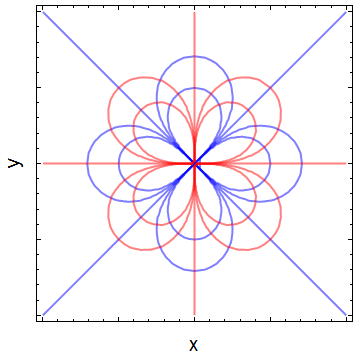
\includegraphics[width=0.75\textwidth]{Figure2.png}
\caption{Plot of level curves of $u'(x,y)$ (in blue) and $v'(x,y)$ (in red) for $f=1/z^2$.}
\label{Fig2}
\end{figure}
Again we see that the level curves are orthogonal therefore we infer that $1/z^2$ is analytic.
\end{enumerate}

\pagebreak

\section{Problem \#4}
To confirm the given identity 
\begin{equation}
\left(\frac{ia-1}{ia+1}\right)^{ib} = \exp[-2b\textnormal{arccot}(a)]
\label{Prob4}
\end{equation}
where $a,b\in\mathbf{C}$, we want to write the fraction inside the parentheses in radial form
. Where for $ia-1$ we have
$$r=\sqrt{a^2+1},\qquad \theta = \textnormal{arccot}(-a)$$
which means that we can write
$$ia-1 = \sqrt{a^2+1}\exp(i\ \textnormal{arccot}(-a))$$
and for $ia+1$ we have
$$r=\sqrt{a^2+1},\qquad \theta = \textnormal{arccot}(a)$$
which implies that
$$ia+1 = \sqrt{a^2+1}\exp(i\textnormal{arccot}(a))$$
So for the identity in equation \ref{Prob4} we have
\begin{align*}
\left(\frac{ia-1}{ia+1}\right)^{ib} &= \left(\frac{\sqrt{a^2+1}\exp(i\textnormal{arccot}(a))}{\sqrt{a^2+1}\exp(i\textnormal{arccot}(-a))}\right)^{ib} \\
&= \left(\frac{\exp(i\textnormal{arccot}(a))}{\exp(i\textnormal{arccot}(-a))}\right)^{ib} \\
&= \left(\exp(i\textnormal{arccot}(a))\exp(-i\ \textnormal{arccot}(-a))\right)^{ib} \\
&= \left(\exp(i(\textnormal{arccot}(a)-\ \textnormal{arccot}(-a)))\right)^{ib} \\
&= \left(\exp({i(\textnormal{arccot}(a)+\ \textnormal{arccot}(a))})\right)^{ib} \\
&= \left(\exp(2i\textnormal{arccot}(a))\right)^{ib} \\
&= \exp\left[(ib)2i\textnormal{arccot}(a)\frac{}{}\right]\\
&= \exp\left[-2b\textnormal{arccot}(a)\frac{}{}\right]
\end{align*}
So we confirmed the identity.

\end{document}

